\subsection{Needle variations}
In the beginning of section 3 we talked about the variations of trajectories, and analyzed those variations \textit{a-posteriori}, trying to describe them. Now we are going to see, so to say, \textit{the elementary (infinitesimal) way of producing said variations.} This will be of course through control variations, not through the variation of initial condition.


\paragraph{Needle variation (fixed interval)}
Let \controlSystem be a control system, $x_0\in\chi$ be an initial condition for eq. \ref{e1.1}, $\tzto\subset\R$ a time interval, $\mu\in\admContr{x_0,t_0,\tzto}$. We then define 
\lista{
	\item \grass{fixed interval needle variation \underline{data}} as a triple $\theta=(\tau_\theta,l_\theta,\omega_\theta)$ for which \lista{
		\item $\tau_\theta\in(t_0,t_1]$
		\item $l_\theta\in\R_{\geq0}$
		\item $\omega_\theta\in U$
	}

	\item the \grass{control variation} of the control $\mu$ associated to the relative fixed interval needle variation data $\theta$ is the map $\mu_\theta$ is the map $mu_\theta:J\times\tzto\fd U$ such that
	\[\mu_\theta = \left\{ \begin{array}{lr}
	\omega_\theta & \mbox{if $t\in[\tau_\theta-s*l_\theta,\tau_\theta]$}\\
	\mut & \mbox{otherwise}.\end{array}
	\right.	\]
	Where $J=[0,s_0]$ is an interval sufficiently small so that $\mu_\theta(s,t)$ is an admissible control for each $s\in J$
	Just to have an idea, this is how the function $\mu_\theta$ can look like for a certain $s>0$
	\begin{figure}[H]
		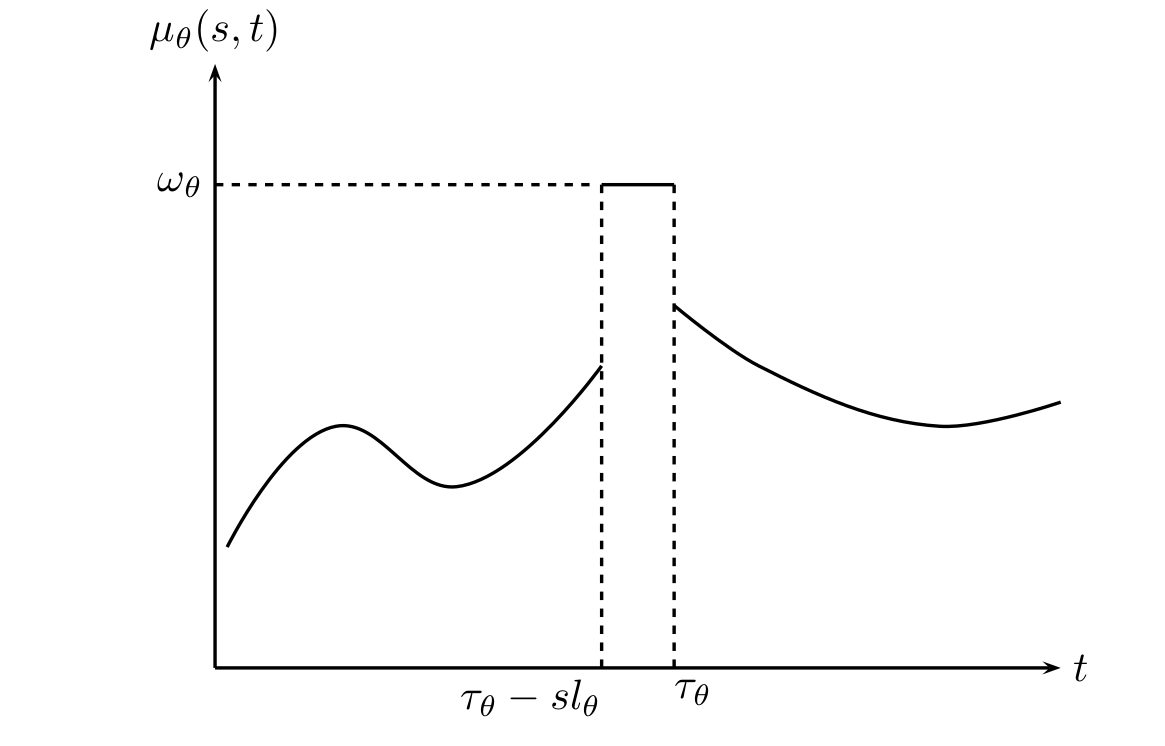
\includegraphics[width=\linewidth]{imgs/needle-variation.png}
		\caption{}
		\label{fig-needle-variation}
	\end{figure}
	\item \grass{fixed interval needle (\textit{infinitesimal})variation} associated with the control $\mu$, the trajectory \trajWinCond{\cdot} and the variation data $\theta$ as a vector of $\R^n$ defined as 
	\[v_\theta = \frac{d}{ds}\bigg|_{s=0} \xi(\mu_\theta(s,\cdot),x_0,t_0,\tau_\theta),\] when such derivative exists
}
This limit exists at almost any instant, since it exists for every instant that is a Lebesgue point for $t\fd f(\trajWinCondMath{t},\mut)$. Before stating this formally, we need the definition of $Leb(\mu,x_0,t_0,t)$: it's the set of Lebesgue points if $\tau\fd f(\trajWinCondMath{\tau},\mu(\tau)), \tau\in(t_0,t)$. Then,

\paragraph[prop 4.9]{Theorem:existence and form of fixed interval needle variations}\mbox{}\\
Let \controlSystem be a control system, $x_0\in\chi$ be an initial condition for eq. \ref{e1.1}, $\tzto\subset\R$ a time interval, $\mu\in\admContr{x_0,t_0,\tzto}$. Let then $\theta=(\tau_\theta,l_\theta,\omega_\theta)$ be a fixed interval needle variation data, with $\tau_\theta\in Leb(\mu,x_0,t_0,t_1)$. Then the fixed interval variation associated with those data exists and it's given by
\[ v_\theta=l_\theta*\bigg(f(\trajWinCondMath{\tau_\theta},\omega_\theta) - f(\trajWinCondMath{\tau_\theta},\mu(\tau_\theta) )  \bigg) \]

\subparagraph[4.10]{Variations and cones} The real importance of this theorem is not only in the fact that it is (almost) always possible to individuate the infinitesimal variation, but also in the fact that those variations form a cone, which is, if one vector represents a variation, then all of the half-line (originating from $0\in\R^n$) given by that vector is made up of fixed interval variations. Formally said, \\\\

\grass{Proposition:} Let \controlSystem be a control system, $x_0\in\chi$ be an initial condition for eq. \ref{e1.1}, $\tzto\subset\R$ a time interval, $\mu\in\admContr{x_0,t_0,\tzto}$. Let then \fivData be a fixed interval needle variation data, with $\tau_\theta\in Leb(\mu,x_0,t_0,t_1)$.\\
Then, the set of fixed interval needle variation associated with the data $\theta$ form a cone.\\\\
\grass{Proof:} It's just enough to say that, if $v_\theta$ is the variation associated with the data \fivData, then, taken a $k\in\R_{\geq0}, kv_\theta$ is the variation associated with the data $k\theta=(\tau_\theta,k*l_\theta,\omega_\theta)$. Using obvious notation, one could then say that $v_{k\theta}=kv_\theta$.\\
It is interesting to note that, in the triple representing the data, only the \textit{"lenght of the disturbance"} gets multiplied by the scalar. This means, that, referring to \ref{fig-needle-variation}, the final control is practically the same. In fact, the actual length of the horizontal step in the figure doesn't really matter, since s tends to zero, and the actual disturbance gets reduced to a (Lebesgue-neglettable) single point in time. \\
The only effect one may obtain is that, given a certain trajectory, the trajectories associated with varied control depart from the undisturbed one at a higher rate with growing s (at least, as long as s is small enough so that one can linearize the effect of control variation), but in the same direction. This is the same exact meaning of the length of the dotted arrows in \ref{fig-variations}.


\subsection{Reachable set}
Let \controlSystem be a control system, $x_0\in\chi$ be an initial condition for eq. \ref{e1.1}, $\tzto\subset\R$ a time interval, $\mu\in\admContr{x_0,t_0,\tzto}$. We then define \lista{
	\item \grass{the reachable set} from $x_0$ at $t_0$ in time $t_1-t_0$ as 
	\[\mathfrak{text}  \]
}